\section{The Idealized Prime+Probe Technique}

The idealized Prime+Probe technique helps to visualize the vulnerability of AES cipher during the 1st Round. To keep things simple, we'll consider an idealized environment in which only the attacking process and the victim encrypting process exists. Also assume that the attacking process will be able to invoke or interrupt the encrypting process at any time. Now since we are talking about triggered encryption, the plaintext is always known.

\begin{center}
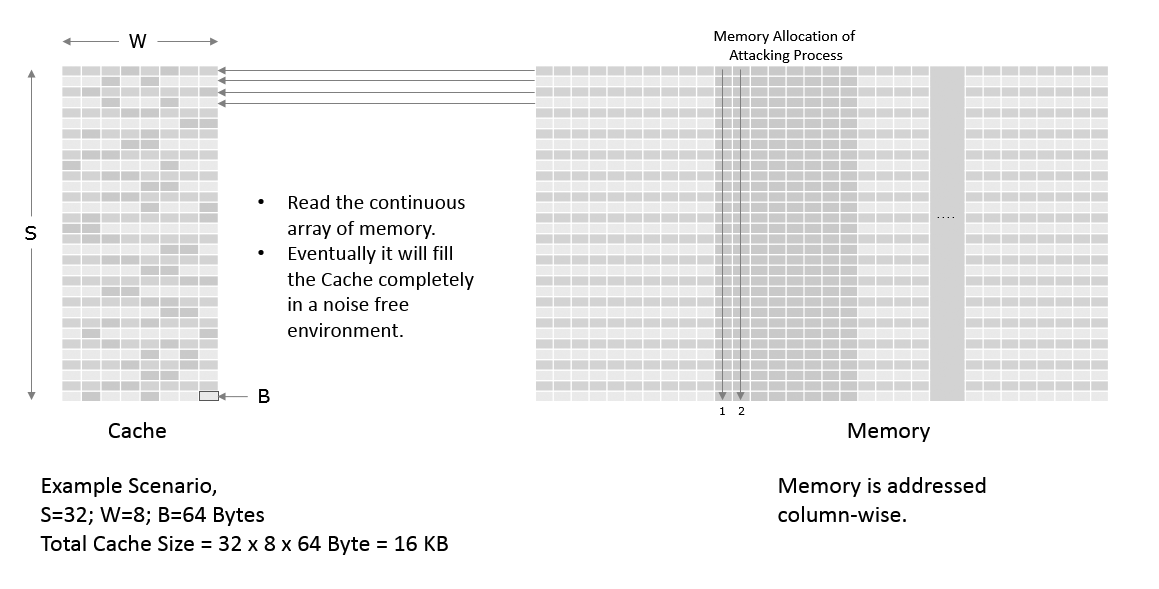
\includegraphics[scale=0.4,natwidth=1159,natheight=589]{psd/filling(new).png}
\captionof{figure}{Demonstration of the Cache filling process. Note that reading continuous array of memory will cause allocation of one block from each cache set.}
\end{center}

\begin{flushleft}
The Prime+Probe technique has the following 3 phases:
\end{flushleft}

\begin{itemize}
\item Prime
\item Trigger
\item Probe
\end{itemize}

\paragraph{Prime}
During the Prime phase, the cache is filled completely by the attacking process. This can be done by allocating a contiguous amount of memory as big as the size of the cache and performing a read on it.

\paragraph{Trigger}
With the cache filled with data of the attacking process, it will trigger an encryption for some known plain text. As the encrypting process reaches the first round and performs table lookup, it is interrupted. An important point to note here is, the model is idealized here to illustrate the susceptibility of the first round. Recovering the AES Encryption Key is not the intent of this paper.

\paragraph{Probe}
After the encrypting process is interrupted just after it performed a table lookup during the first round, the Prime step is done again, i.e. the cache is filled again. But this time, a clock is maintained to determine a cache miss. Before the Trigger phase, the cache was completely filled by attacker's data. But after that Trigger phase, one block of the 
Lookup table $T_i$ is now in the cache due to lookup operation. So all but that block will suffer a cache miss.

Observing the position of the cache miss, the attacking process can identify which block of $T_i$ was accessed since it was assumed that Lookup Tables $T_i$ are congruent with the cache. Since size of \emph{memory block} is 64 Bytes in most cases, each \emph{memory block} holds 16 entry of the Lookup Table. So for example, if 7th block of $T_0$ was accessed, one can conclude the index $x_0^{(1)}$ was somewhat between 0x60 and 0x6F, i.e. the high nibble is 0x6. We know

\begin{align*}
x_0^{(1)}=x_0^{(0)} \oplus k_0^{(0)}
\end{align*}

\begin{algorithm}
\caption{Abstract procedure for capturing half of the Key during the first round}
\label{Abstract procedure for capturing half of the Key during the First Round}
\begin{algorithmic}[1]
	\State triggerEncryption()
	\For{$i \gets 0$ to $15$}
		\State fillCache()
		\State haltEncryption()
		\State $j \gets$ missedBlockIndex()
		\State $j \gets j\ll 4$
		\State $k_i^{(0)} \gets j \oplus x_i^{(0)}$\Comment{$k_i^{(0)}$ and $x_i^{(0)}$ resemble i-th Byte of the key and known plaintext respectively}
	\EndFor
\end{algorithmic}
\end{algorithm}

Here $x_0^{(0)}$ is the 1st Byte of the plaintext and $k_0^{(0)}$ is the 1st Byte of the Encryption Key. Now, since addition and subtraction in Galois Field are the same XOR operation, rearranging the equation yields:

\begin{align*}
k_0^{(0)}=x_0^{(0)} \oplus x_0^{(1)}
\end{align*}

knowing $x_0^{(0)}$ and the high nibble of $x_0^{(1)}$, one can compute the high nibble of the first Byte of the Encryption Key by a simple XOR operation. Proceeding this way for every Bytes $x_i^{(1)}$ for $i=0,1,2,...,15$, one can  dig up half of the Encryption Key. The idealized procedure is summarized in algorithm 1.
